%!TEX root = ../Main.tex

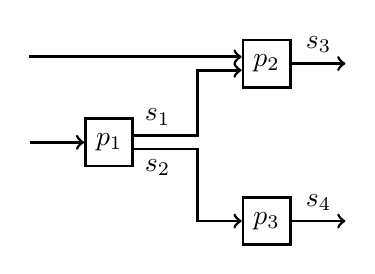
\begin{tikzpicture}[line width = 1pt,
                    process/.style    = {rectangle, draw, fill = white, minimum size = 0.6cm, inner sep = 0pt, align = center}
                    ]
    % \draw (0, 10) to[grid with coordinates] (18, 18);

    \node[process] (p1) at (0, 1) {$p_1$};
    \node[process] (p2) at (2, 2) {$p_2$};
    \node[process] (p3) at (2, 0) {$p_3$};

    \draw[<-] (p1) -- ++ (180:1cm);
    \draw[->] (p1.15) node[anchor = south west] {$s_1$} -- ++ (0:0.8cm) |- (p2.195);
    \draw[->] (p1.345) node[anchor = north west] {$s_2$}-- ++ (0:0.8cm) |- (p3);
    \draw[<-] (p2.165) -- ++ (180:2.7cm);
    \draw[->] (p2) -- ++ (0:1cm) node[anchor = south, midway] {$s_3$};
    \draw[->] (p3) -- ++ (0:1cm) node[anchor = south, midway] {$s_4$};;
\end{tikzpicture} 